\documentclass{cslthse-msc}
\setcounter{tocdepth}{4}
\setcounter{secnumdepth}{4}
\usepackage[utf8]{inputenc}
\usepackage[english]{babel}
\usepackage{amsmath}
\usepackage{amsfonts}
\usepackage{amssymb}
\usepackage{amsthm}
%\usepackage{makeidx}
\usepackage{graphicx}
\usepackage[titletoc, header, page]{appendix}
\usepackage{todo}
\usepackage{float}
\usepackage[hidelinks]{hyperref}
\usepackage{wrapfig}
\usepackage[within=none]{caption}
\usepackage{pdfpages}
\usepackage{svg}
\usepackage{listings}
\usepackage{color}
\newcommand{\hilight}[1]{\colorbox{yellow}{#1}}

\definecolor{mygreen}{rgb}{0,0.6,0}
\definecolor{mygray}{rgb}{0.5,0.5,0.5}
\definecolor{mymauve}{rgb}{0.58,0,0.82}
\usepackage{colortbl}
  \definecolor{Lightgray}{RGB}{235,235,235}

\lstset{
breaklines=true,
language=SQL,
numbers=left,
numbersep=5pt,
numberstyle=\tiny\color{mygray},
frame=single,
basicstyle=\footnotesize,
captionpos=b
}
\newcommand{\bex}{BeX\textsuperscript{\textregistered}}
\renewcommand{\lstlistingname}{Algorithm}% Listing -> Algorithm
\renewcommand{\lstlistlistingname}{List of \lstlistingname s}% List of Listings -> List of Algorithms



\author{
	Alexander Söderberg \\
	{\normalsize \href{mailto:email@alexandersoderberg.com}{\texttt{email@alexandersoderberg.com}}}
	\and
	Max Åberg \\
    {\normalsize \href{mailto:aaberg.max@gmail.com}{\texttt{aaberg.max@gmail.com}}}
}

\title{Optimizing business intelligence
extraction speed from an
ERP-system’s database}
\subtitle{Master Thesis}
\company{Perfect IT BeX\textsuperscript{\textregistered} AB}
\supervisors{Lennart Söderberg, \href{mailto:lennart@perfectit.se}{\texttt{lennart@perfectit.se}}}{Alma Orucevic Alagic, \href{mailto:alma@cs.lth.se}{\texttt{alma@cs.lth.se}}}
\examiner{Per Andersson, \href{mailto:per.andersson@cs.lth.se}{\texttt{per.andersson@cs.lth.se}}}

\date{\today}

\acknowledgements{
\todo{Skriv acknowledgments}
}

\theabstract{
\todo {Skriv abstract}

}

\keywords{MSc, MsSQL, ERP, Optimization}

%% Only used to display font sizes
\makeatletter
\newcommand\thefontsize[1]{{#1 \f@size pt\par}}
\makeatother
%%%%%%%%%%


\begin{document}
\makefrontmatter

\chapter[Introduction]{Introduction}
2014 was the year of the cloud. Software companies strived to make their services cloud based in order to meet the increasing demands from the market of availability and reliability. 	
In today's businesses there's high demand for accurate and up-to-date business intelligence (henceforth referred to as BI).

\chapter{Background}\label{sec:background}

\section{Background}
Perfect It BeX AB was founded by Lennart Söderberg and Niklas Lindgren in 2007. In the beginning they made business extensions such as B2B, e-commerce and retail for the Microsoft Navision ERP. Eventually they started development of their own ERP-system to accommodate their extensions since they felt limited buy the technologies on which Navision was based. In 2010 they released three products; \bex Online, \bex Retail, and \bex B2B. \bex Online is the main product on which the other products rely. It is a completely cloud-based ERP-system specialized for the retail industry. The main functionality in \bex Online are:

\begin{itemize}
\item Financial tools
\item Sales administration \& handling
\item Purchase handling
\item Inventory and Warehousing
\item History and Business Reports
\end{itemize}

In recent years, Lennart and Niklas have felt an increasing demand from customers for better business intelligence capabilities. In response to this they have improved the Business Report functionality in BeX Online, to be able to give a wider range of different financial key values. According to Lennart, being able to offer their customers tools enabling for good business intelligence, is key to staying competitive. Therefore, they want to develop these tools further to make them better and to include more functionality. However, they have noticed that generating some of the reports can take a relatively long time, especially for their bigger clients whose system's have a lot of data.

\section{Problem description}
Perfect It BeX AB has ordered this master thesis to investigate how to increase the generation speed of the business intelligence-reports and to implement a solution that increases this speed.

\section{Thesis Goals} \label{sec:goals}
The goal of this thesis is to examine, test the feasibility and implement a solution for speeding up the generation of BI reports in Perfect IT \bex AB's product \bex Online. To be able to speed up the BI report generation an optimization needs to be done. The optimization needs to be versatile to handle the current system, to handle new functionality and also future company growth. Hence, the optimization needs to be scalable. Taking in to account that Perfect IT \bex has one physical server, the scalability should be vertically\cite{scalability} since the company will provide the system to more clients in the future.\\\\
In order to make the above optimization possible, the following goals have been established:
\begin{enumerate}
\item Acquire knowledge about database optimization in general.
\item The current processes behind generation of the BI-reports must be identified and mapped in Perfect IT \bex AB.
\item Analyze and identify bottle-necks and inefficiencies.
\item Solution approach research to solve the problems identified in the analysis. The research will consider as many options as possible to find a long-term solution.
\item Analyze solution approaches to decide which of them are a best fit and should be used to reach the goal.
\item Implement the solution in \bex Online and a final analysis should be performed to determine if the goal was met.
\end{enumerate}
  
\section{Scope} \label{sec:scope}
According to Nevarez\cite{Nevarez} the main areas of investigation while trying to optimize an existing database for speed are:
\begin{itemize}
\item Query tuning
\item Execution plan tuning
\item Index tuning
\item Database execution statistics
\item In-Memory OLTP
\item Plan caching
\end{itemize}
Due to the limited time frame of this thesis, all of these areas won't be explored. With respect to this and the company's preferences the following focus areas were decided upon: Query tuning, index tuning and "In-Memory OLTP"-solutions.

\section{Limitations}

The objective is primarily to increase the speed of the ERP-system's business intelligence reporting module by optimizing the database. The database is used by all parts of \bex Online. This means that the following limitations to the developed solution must be in place.

\begin{itemize}
\item The solution must not affect any functionality in \bex Online.
\item The solution must not decrease performance in other \bex Online functionality.
\item The solution must work with the current implementation of \bex Online Back-end.
\end{itemize}

\section{Related Work}

\section{Contributions}

\chapter{Research Questions \& Methodology}

\section{Research Questions}
The research questions of this thesis were formulated in relation to the thesis goals in section \ref{sec:goals} and the scope in section \ref{sec:scope}. The thesis is formed to explain and answer the following research questions:
\begin{itemize}
\item	How does the current system system work and what are the bottle-necks?
\item 	How does index fragmentation, query tuning and ''In-memory OLTP'' work in general?
\item	What optimization solutions are best-fit and why?	
\item 	Is the proposed solution versatile and scalable so that it is a long-term solution?
\item	How can the proposed solution be implemented in Perfect IT \bex AB's current system?
\end{itemize}
\section{Methodology}
This thesis is of a problem solving nature and should continuously adapt to changing conditions. The methodology used should therefore preferably be flexible. A methodology that provides valuable support and is intended to improve something while studying it is action research\cite{robson}. Action research begins with an observation phase that identifies and clarifies the problems that are present, for this thesis that is presented in chapter \ref{sec:background}. In chapter \ref{sec:proposedsoluton} the next step in action research is stated, a proposed solution to the problem(s).\\

After implementing the proposed solution an important, but often neglected, phase is performed namely the evaluation. The evaluation is made to verify the implementation in its context, to analyze and reflect on how it works in its integration. The whole action research is an iterative process and is based on the evaluation. Accordingly to Höst et al.\cite{regnell} an evaluation is hard to keep unbiased, since the ones doing the critical evaluation are also the ones that performed the research. To counter an unbiased evaluation, some evaluation criteria were established based on the above mentioned goals in section \ref{sec:goals}. To ensure that all of the stakeholders goals are met this thesis will on a regular basis be reviewed both by supervisors at Perfect IT and at LTH.

\section{Work}
First of all an acquaintance of Perfect IT \bex AB's system needed to be established. In conjunction with the examination of the current system and its parts a literature research was performed. The area this research treats is extensively and the research done is almost indefinite. Therefore the literature research scope needed to be narrowed with its base in the currents systems examination.\\\\    
To find the literature and related work Engineering Village\cite{Enginvillage} and Google Scholar\cite{Googlescholar} together with DBLP\cite{DBLP} was used. A lot of time was dedicated to find relevant literature and information for this thesis and at the same time examine if the ideas established during the system examination phase were possible, and solid, solutions.\\\\
Using the paper written by Gruian and Lekebjer on formatting a master’s thesis\cite{Reportmall} and guidelines from the book by Regnell et al.\cite{regnell} the initial work on the master thesis report was conducted. 
\todo{to be continued\ldots}

\chapter{Approach}

\section{Technical System Description}
Perfect IT delivers web-based business systems and services specialized for the retail industry. The \bex Online ERP-system is distributed as a SaaS-solution and all clients share servers which makes it a true cloud based service. The clients access \bex Online's front-end through a web browser. \bex Retail and \bex B2B are connected directly to \bex Online's back-end.
The database for \bex Online is a Microsoft Server 2014 Web Edition.
\begin{figure}[H]
\vspace{-15pt}
  \begin{center}
    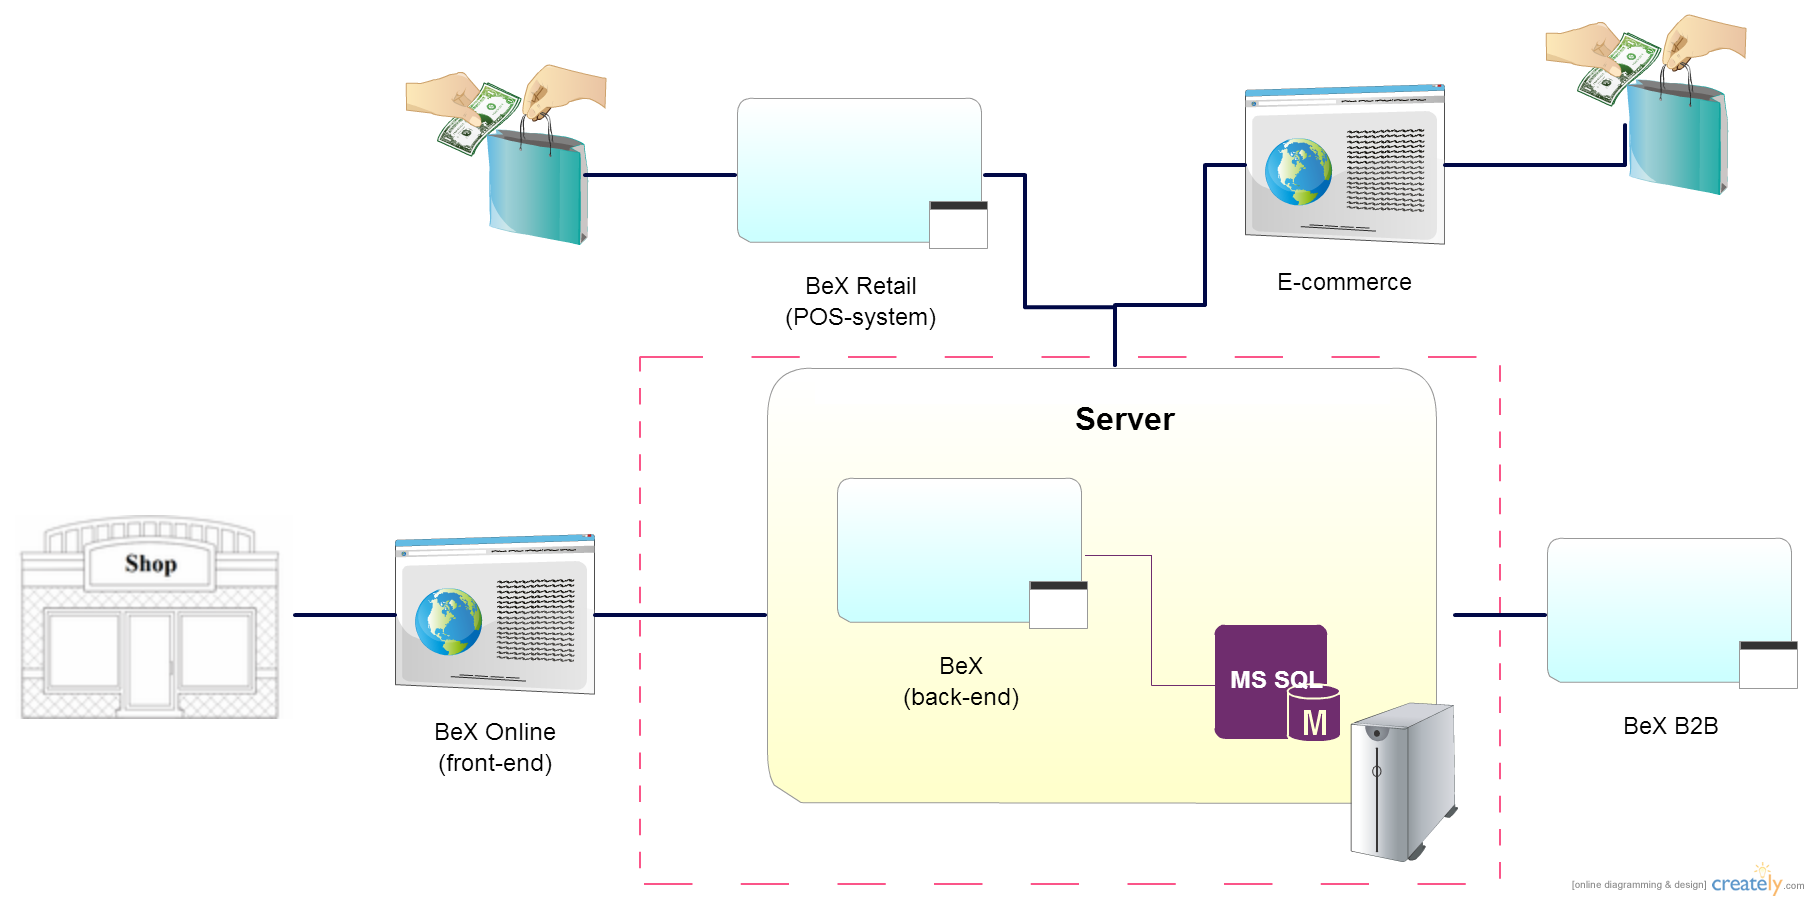
\includegraphics[scale=0.3]{Systemdesc.png}
  \end{center}
  \caption{Context diagram of Perfect IT's system}
  \label{context}
  \vspace{-15pt}
\end{figure}
\noindent The dashed section in Figure~\ref{context} are the components that are of the most interest for this thesis and will be more thoroughly described than the other system components.

\subsection{Components}


\subsubsection{Server}
Currently all the clients instances of /bex Online are placed on a single server hosted by a third party hosting company. This server also hosts the database system.
The technical specification of the server is:
\begin{table}[H]
\begin{center}
\begin{tabular}{l l}
OS: & Windows Server 2012 Standard 64-bit\\
CPU: & Intel(R) Xeon(R) CPU E5-2440 @ 2.40 GHz 64-bit based\\
RAM: & 64 GB \\
HD: & 500 GB Disk drive
\end{tabular}
\end{center}
\end{table}

\subsubsection{\bex Online}
\bex Online is a web based system and has a front-end built with HTML5, CSS and JavaScript and a back-end written in C\# and .net with Webforms.
Every client have their own instance of the system \todo{deeper description}

\subsubsection{Database}
Microsoft SQL Server Web edition, 64GB Ram, Maximum data capacity: 524 PB, Maximum CPU capacity < 4 socket or 16 cores. All clients are on the same SQL Server 2014-license but have their own unique instance of the database-system with only their data.  Perfect IT has has around \hilight{40} clients connected to the servers database, all with different sizes of data ranging from approximately \hilight{5GB data to approximately 60GB} data. The database is an RDBMS and is run on a Microsoft SQL Server 2014-license using OLTP and the size of all the clients databases together are approximately \hilight{350GB}.

\paragraph*{Tables}\mbox{}\\\\
For this thesis Perfect It BeX AB has made available a copy of one of their biggest clients database. To ensure the clients privacy, and the privacy of the clients customers, all sensitive data has been removed. \\ 
The default schema is called \textit{dbo} and consists of a total of 254 tables, including some views for big data queries. Many tables are large, considering the amount of rows, where the largest consists of approximately 10.5$\times 10^6$ rows and 80 columns. This table stores the data associated with every business transaction made by the system from the start of using this system. There are also empty tables, \hilight{usage?}, that \ldots. The tables form a complex relation to each other and the references are many (as seen in this \href{https://drive.google.com/file/d/0B1IYTmE2hnD-eGQ0N2tvYXZNNVE/view?usp=sharing}{\textcolor{blue}{link}}). In the visualized database reference schema there are tables not referencing any tables at all, \hilight{why?}.\\\\ There are also tables needed by third party applications and API's that also are stored in the database and can be seen in the bottom part of the visualized database reference schema mentioned above (\hilight{maybe the answer to the no reference question above?}). Some, \hilight{why not all?} of the BI reports have their own tables in the database, \hilight{why?}.

\paragraph*{Stored procedures}\mbox{}\\\\ 
Stored procedures are subroutines that are available to applications that access relational database systems. Stored procedures are used as centralized logic and can therefore be used by all applications that share the system. These subroutines can include both SQL statements and host language statements, meaning that it can exist external procedures that has nothing to do with SQL. Often extensive and complex SQL queries, that require a lot of processing and are often being used, are moved to stored procedures for reuse\cite{StoredProcedures}. It's important to know that Stored procedures both bring advantages, e.g. Stored procedures are cached, and drawbacks, e.g. Stored procedure code is not as robust as app code. Subroutines such as Stored procedures should therefore only be used when and if the implementer possess a deep knowledge of the system that is to be affected. It's for example bad practice to store all procedures as Stored procedures for the benefit of the cache-utilization.\\\\
The database in this thesis had a total of 59 Stored procedures treating repetitive procedures by the database mainly for the sales part of the system and the BI reports (there's also a subroutine for locking crucial information, with respect to concurrent execution). These subroutines do not contain any host language statements and/or external procedures, but only consists of complex SQL statements. They are present in the system, as mentioned above, to make the execution and processing less demanding, as they are often used in \bex Online.

 
\section{Theory}
In order to understand why a database might not perform optimally, the following theory was used.

\subsection{Index Fragmentation}
Index fragmentation is one of the most common problems in a relational database. Two kinds of fragmentation can occur, internal index fragmentation and external index fragmentation. The easiest way to explain index fragmentation is by imagining the SQL database as a phone book. At the very end of the book you have a few pages containing a table with indexes of all the entries sorted by last name. This is fine in a static environment such as a phone book but what happens in a dynamic environment?
Since people can be added to the phone book there must be space available after each column in the index, as well as in the pages in the phone book. This is called the \emph{fill factor}. A page can still run out of space and when this happens SQL Server has to add a new page, but it it can't add it at the correct place because the book is already bound. So, it adds blank pages at the very end. This causes two problems, pages with a lot of unused space and pages that are out of order. The first problem is what is referred to as \emph{Internal Fragmentation} and the second is \emph{External Fragmentation}. Internal fragmentation will of course also occur when deleting entries since that leaves "blank space" on the page.\cite{Ozar12}

\subsubsection{Why is this bad for performance?}
At first, internal fragmentation might seem like a good thing. If the phone book has a lot of blank space on every page to start with, adding entries would be super easy and there would be no need for adding more pages later, causing external fragmentation. This is true, but when the number of extra pages needed in the phone book to allow for a lot of blank space is considered, the inefficiency of it becomes apparent. Going through a 100\% filled 1000 page phone book is much faster than a 90\% full 1100 page phone book. So in this example, every time SQL Server needs to scan the index, it would take 10\% longer. Another problem is that the lowest unit for caching in SQL Server is not a record, but a single page, which means that all the empty space must be cached as well. \\

External fragmentation often makes reading the database non-sequential, i.e it cannot be read in order but must be read in random order. This is especially bad in classic magnetic hard drives where the reader head must move around to multiple locations on the drive. Some magnetic hard drives only get 1\% of their sequential reading speed when performing random reads.\cite{Toshiba12}

\subsubsection{Measuring fragmentation}
In Al-Farooque Shubho's article "Top 10 ways to optimize data access in SQL Server"\cite{Shubho09} he explains how to measure if index fragmentation has occurred. By executing the script on page \pageref{lst:fragalg} in Algorithm \ref{See DB-Fragmentation}, index fragmentation is analyzed on every table in the database and presented in a table with an internal and external fragmentation value. \\

According to Shubho, only tables with an internal fragmentation value of less than 75 and/or an external fragmentation value of more than 10 should be considered as fragmented, which this code takes into account.

\subsubsection{Reorganize vs. Rebuild}\mbox{}\\
Both rebuilding and reorganizing are built-in operations in SQL-Server 2014. These are two different operations that both reduce the fragmentation of the indexes. Reorganizing is the more lightweight of the two operations. It fixes the indexes as well as physical reordering of pages and applies any previously set fill factors. Rebuilding builds up a completely new structure for the index. It also allows for a new fill factor.\\
The advantage with reorganizing over rebuilding is that it can be aborted midway, while a rebuild must roll-back after an abort. Usually, in most SQL-systems, a rebuild can't be done while the SQL-server is online. This can be done in MS SQL Server Enterprise edition\cite{Little13}.

\subsubsection{Is it always a good idea to fix fragmentation?}
According to Brent Ozar\cite{Ozar12} fixing fragmentation can cause more damage than keeping fragmented indexes. Often administrators try to fix fragmentation by using a low fill factor, say 50\%. This would mean that half of every page would be blank, which would make writing really fast. Reading however, would be twice as slow. Another common mistake is to rebuild every single index in the database, even though some tables might not had a single write since the last time. This is a problem because defragmenting indexes causes SQL Server to write to the transaction log. The bigger a log is, the longer log backups and restores take.\\\\
Another important factor is that external fragmentation mostly causes problems when the database is stored in disc, since classical hard drives are slow at random reading. If the database is instead stored in memory, which is almost as fast at random reading as sequential reading, external fragmentation won't be as big a issue.

\subsection{Query optimization}
When talking about query optimization one imagines that the logic in the SQL statements are altered and optimized. Even if this is true, by tuning the actual SQL statements an optimization can be accomplished, it's done with respect to the execution plan. Query optimization can also been seen as mapping of the logical query operations to physical operations that the execution engine can execute.It does this by implementing a number of algorithms, which the query optimizer must choose from when formulating an execution plan. In summary a query optimization is actually a strategic manner to optimize the execution functionality of the execution engine\cite{Nevarez}. \\\\ 
The purpose of the query optimization is to provide a good enough and hopefully optimal execution plan. In order to do so a query must go through a query-processing process as can be viewed in Figure~\ref{fig:qpp}. The query-processing starts with a simplification of tree representation that is sent from the Algebrizer, which checks the syntax and appropriate bindings of the SQL statement(s). There are 4 stages in the query-processing that return an execution plan and if the simplification of the logic tree representation qualifies as a trivial plan a trivial execution plan is returned and the optimization process ends immediately. Otherwise a full optimization process will be run in up to three stages and an execution plan may be created at the end of any of these stages. All the alternatives the full optimization returns are stored and evaluated by the SQL server based on the cost. The whole optimization is a cost/benefit trade-off regarding the query optimization time. The number of varying plans can easily rise, an effect known as the combinatorial explosion\cite{combo}, and the optimization will therefore not be feasible as it takes too long. Therefore during this full optimization process the query optimizer uses statistics, transformation rules, heuristics and cost estimations to limit and assure the quality of the executions plans that are returned.\\\\ 
As the query optimizer limits the available alternatives two problems arise. The entire search space is not evaluated and the chosen execution plan is therefore impossible to prove that it's the most optimal one. So the query optimizers utmost important functionality lies in considering the plans that are of low cost. Which brings us to another major technical challenge, accurate estimations. The quality of the plan that is chosen is only as good as the accuracy of the estimation. According to Nevarez\cite{Nevarez} the estimations are inherently inexact and do not consider the environments hardware conditions.
\begin{figure}[H] 
\begin{center}
    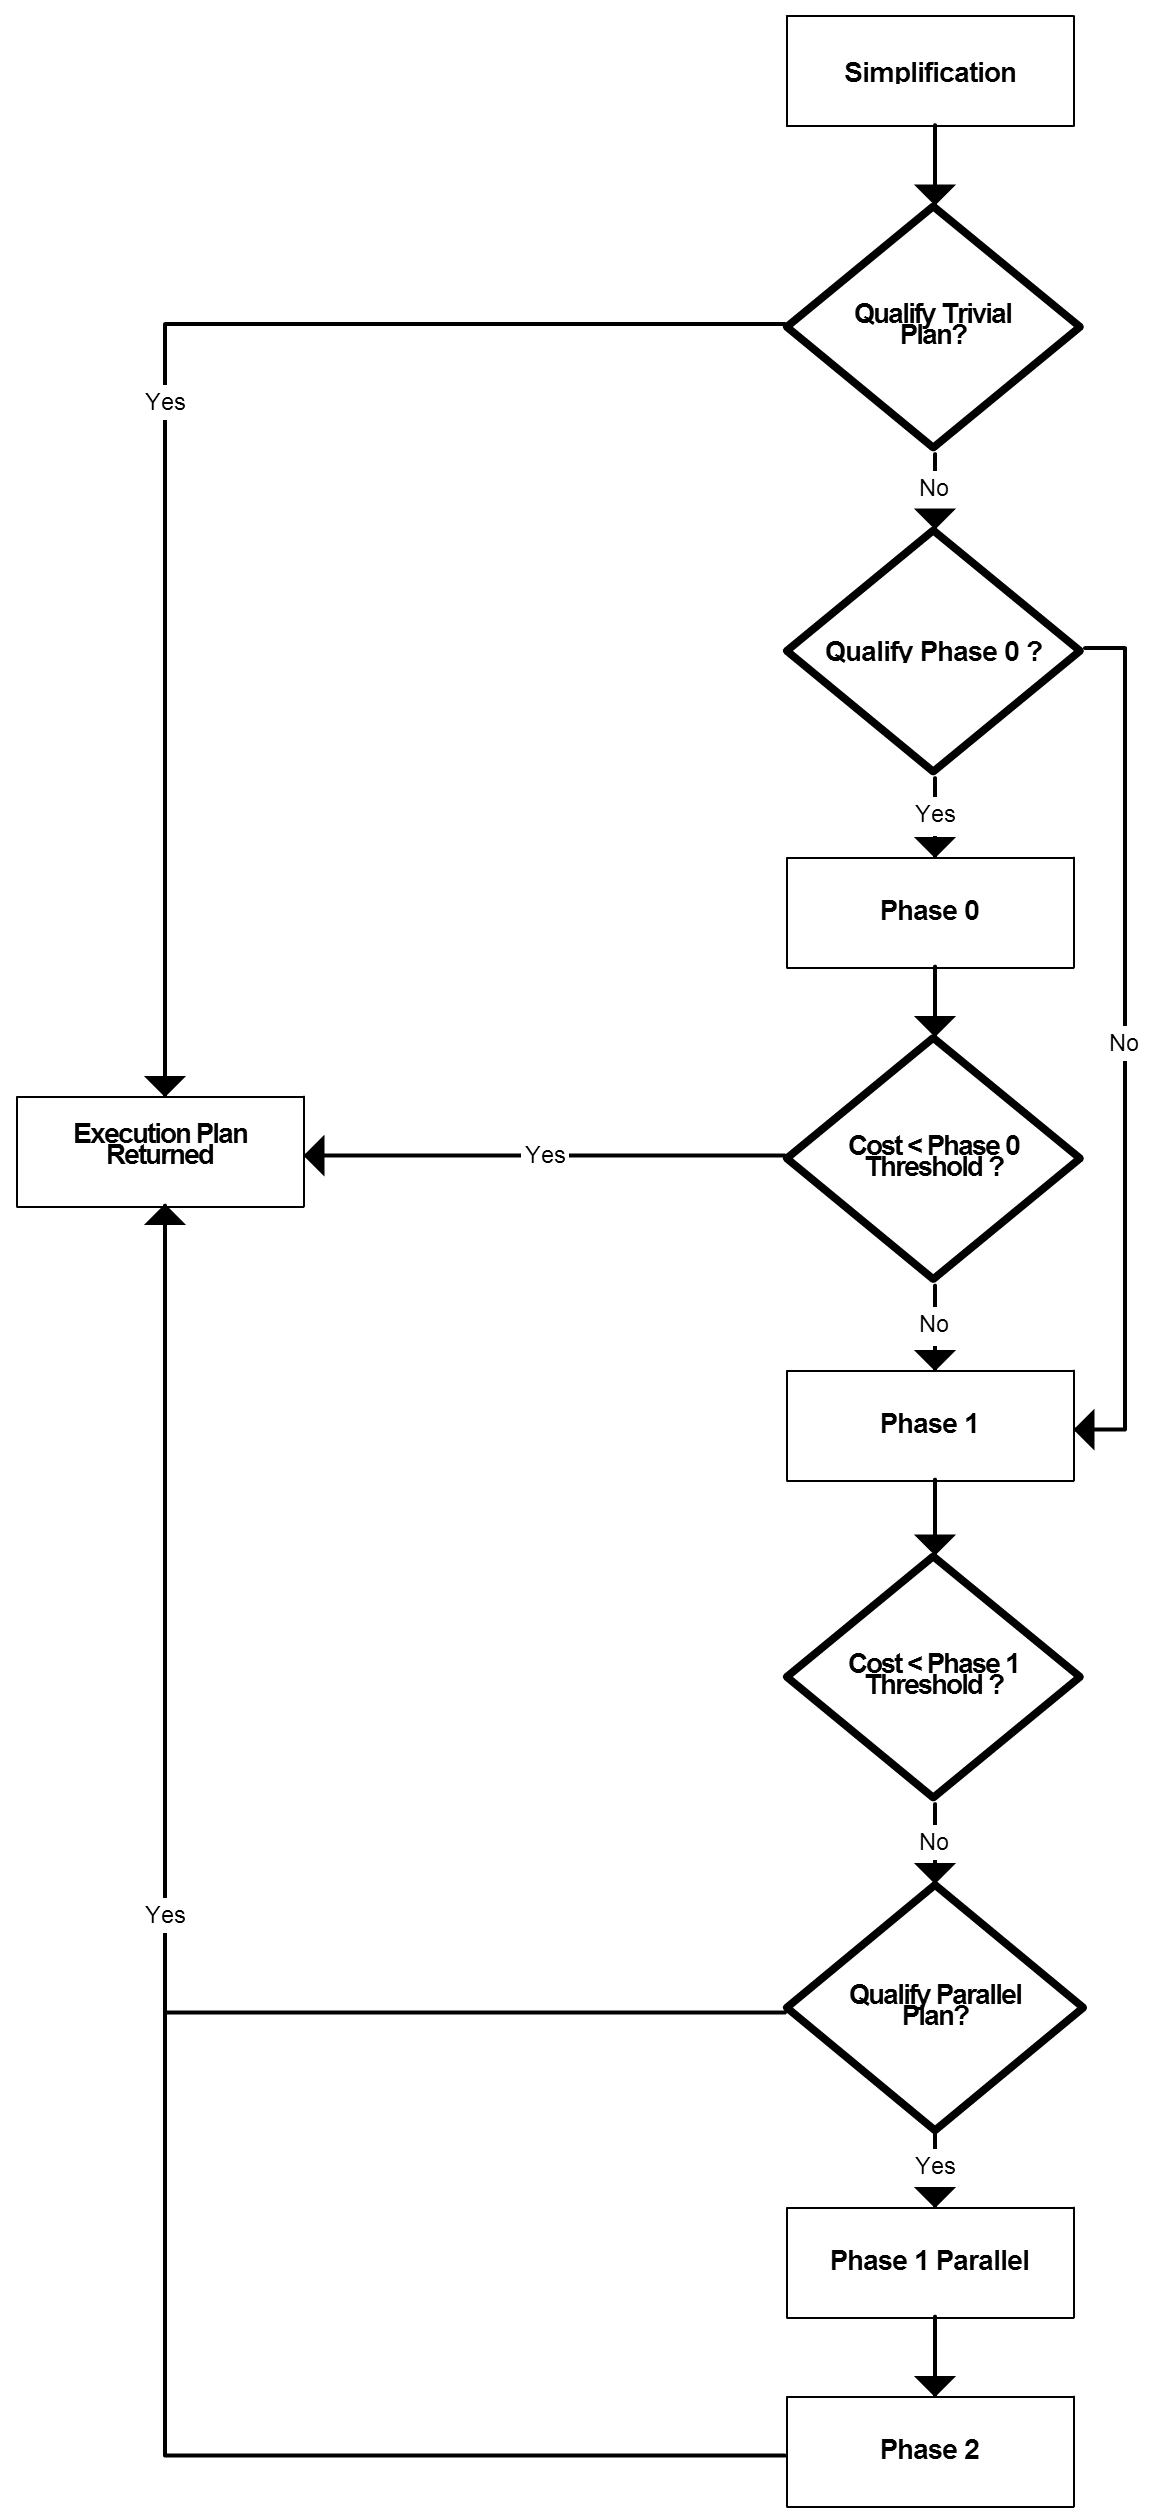
\includegraphics[scale=0.3]{Optimization-process.png}
  \end{center}
  \vspace{-20pt}
  \caption{The query-processing process}
  \label{fig:qpp}
  \vspace{-10pt}
\end{figure} 
\noindent As an example the cost model assumes that every query's data is read from disk and not from memory (cold cach). In addition some operations are not covered by the mathematical model, leading to that the query optimizer has to resort to guessing logic and/or heuristics to deal with such situations. 

\subsubsection{Query tuning}
In order the optimize the process explained above there are numerous areas that can be altered. One can dive in to the actual SQL statements and try to break down complex queries, optimize join ordering etc. Besides altering the SQL statements the workload sent to the query optimizer can be optimized in several ways. Chaudhuri et al. state that compressing the size of a workload, which is a set of SQL statements, improves a systems scalability and illustrates its effectiveness in index selection and approximate query processing\cite{compressing}. Furthermore, major database vendors have focused on releasing automated physical database design tools that reduce the total cost of a workload. An essential assumption of these tools is that the workload consists of a set of SQL statements with no internal ordering. Agrawal et al. state that the workload in itself isn't the most promising aspect of workload optimization, but that the workload can be treated as a sequence which broadens the usage of the above mentioned tools\cite{automatic}.

\paragraph*{Join ordering}\mbox{}\\\\
\cite{join}
\begin{table}[H]
\centering 
\begin{tabular}{ l l l }
  Trees & Left-Deep Trees (n!) & Bushy Trees (2n-2)!/(n-1)! \\\hline
  2 & 2 & 2 \\\hline
  3 & 6 & 12 \\\hline
  4 & 24 & 120 \\\hline
  5 & 120 & 1 680 \\\hline
  6 & 720 & 30 240 \\\hline
  7 & 5 040 & 665 280 \\\hline
  8 & 40 320 & 17 297 280 \\\hline
  9 & 362 880 & 518 918 400 \\\hline
  10 & 3 628 800 & 17 643 225 600 \\\hline
  11 & 39 916 800 & 670 444 572 800 \\\hline
  12 & 479 001 600 & 28 158 588 057 600 \\
\end{tabular}
\caption {Possible join orders for Left-Deep and Bushy trees}
\label{table:join}
\end{table}
\paragraph*{Query break down}\mbox{}\\\\   

\subsection{In-Memory Database Technology}
Relational database management systems were originally designed in the late 70's\cite{Nevarez}. Because of this, they are designed with the assumption that memory is limited, expensive and that the size of the database is many times larger than the main memory. Today, memory is relatively cheap and it is possible to have hundreds of gigabytes of memory in a single server. This makes it possible to put even large databases, completely in memory. In Vizard's article\cite{Vizard12} it is said that having a database completely in-memory can make it a thousand times faster.

\subsubsection{Hekaton}
Microsoft SQL Server 2014 comes with an In-Memory OLTP database engine called Hekaton. Hekaton, which is only available in the enterprise edition, improves performance in three major architecture areas: Optimization for main memory access, compiling procedures to native code, and latches and lock elimination. The core architecture of Hekaton is a Bw-tree design\cite{Levandoski14}. A Bw-tree is a new design of the classical B-tree which supports high performance in both access to individual keys and key-sequential access to subranges of keys. The Bw-tree is designed for the new hardware environment in two main ways. 
\begin{enumerate}
\item The Bw-tree is latch-free, which is critical for performance when using multi-core systems where latches otherwise are common.
\item Updating cache memory in place in multi-core systems usually results in costly cache invalidations, limiting performance. By performing "delta" updates, the Bw-tree avoids in-place updates which reduces invalidations and preserves previously cached page data.
\end{enumerate} 
The Hekaton engine is not a separate database system, it is fully integrated into SQL Server. A user can declare a table in a current database to be memory-optimized, and the Hekaton engine will store it in main memory and manage it. A Hekaton table can use two different kinds of indexes. Hash indexes and Range indexes.  Even though Hekaton uses very different internal concepts and implementations it still ensures that all transactions have ACID-properties. \\
A big drawback of using Hekaton tables is that the table architecture cannot be altered without recreating the table. This means that in order to change the columns in a table or it's indexing settings, the table must be dropped and then rebuilt from scratch.

\paragraph*{Stored procedures in Hekaton}\mbox{}\\\\ 
Hekaton uses the SQL Query Optimizer to produce an efficient query plan. This plane is then compiled into native C code and loaded as DLLs into the SQL Server process. This compilation happens on SQL Server start.
When a procedure is saved as a natively  compiled stored procedure it locks all the tables that it uses. This is because such procedures must be schema bound, i.e all tables referenced by a procedure can't be dropped. If this is considered together with the the limitation mentioned above regarding changing of a table architecture, the following process would be required in order to change e.g. a Hekaton table's columns\cite{Nevarez}.
\begin{enumerate}
\item Drop the procedures referencing the table.
\item Store the data in the Hekaton in a temporary table.
\item Drop the Hekaton table.
\item Rebuild the Hekaton table with the new columns.
\item Reload the data from the temporary table into the new Hekaton table. 
\item Recreate the stored procedures.
\end{enumerate}


\section{Analysis}

\subsection{Index fragmentation}
By using the script from the theory the following index fragmentation values were produced. The table names and index names has been changed due to confidentiality.

\begin{table}[H]
\begin{center}
\begin{tabular}{|l|l|l|l|}
\hline
Table name & Index name & External fragmentation & Internal fragmentation \\ \hline 
1  & a & 100         & 74,05485545 \\ \hline
2  & b & 100         & 72,6278725  \\ \hline
3  & c & 100         & 58,68544601 \\ \hline
4  & d & 100         & 70,17500618 \\ \hline
5  & e & 100         & 67,92068199 \\ \hline
6  & f & 100         & 58,46971831 \\ \hline
7  & g & 100         & 50,03706449 \\ \hline
8  & h & 99,48535234 & 57,89085743 \\ \hline
9  & i & 96,11111111 & 73,69038794 \\ \hline
10 & j & 94,44444444 & 70,63737336 \\ \hline
11 & k & 90,59325223 & 52,81183593 \\ \hline
12 & l & 89,13043478 & 65,47550037 \\ \hline
13 & m & 86,99186992 & 65,83502595 \\ \hline
14 & n & 85,71428571 & 47,9579318  \\ \hline
15 & o & 78,98550725 & 57,05273042 \\ \hline
16 & p & 77,77777778 & 56,54531752 \\ \hline
17 & q & 75          & 48,44946874 \\ \hline
18 & r & 73,35790885 & 62,85373116 \\ \hline
19 & j & 71,30559541 & 64,10468248 \\ \hline
20 & s & 69,67213115 & 69,75221151 \\ \hline
21 & m & 68,46173667 & 65,69195701 \\ \hline
22 & t & 67,79506955 & 65,90287868 \\ \hline
23 & u & 66,66666667 & 49,09809736 \\ \hline
24 & v & 50          & 74,49962936 \\ \hline
25 & w & 50          & 53,43464295 \\ \hline
26 & x & 50          & 54,92957746 \\ \hline
27 & y & 50          & 41,83552014 \\ \hline
28 & z & 36,59652333 & 72,06630838 \\ \hline
29 & å & 33,5729147  & 73,20072894 \\ \hline
\end{tabular}
\caption{Results from index fragmentation search}
\end{center}
\end{table}

This shows that a some of the indexes used have well over an external fragmentation value of 10. The internal fragmentation value is also bad at some of the indexes (i.e less than 75).

\chapter{Proposed Solution}\label{sec:proposedsoluton}

\section{Solution Introduction}

\section{Integration}

\chapter{Software Development \& Testing}

\chapter{Discussion}

\chapter{Conclusions}
\addcontentsline{toc}{chapter}{Bibliography}
\bibliographystyle{ieeetr}

\bibliography{MyMSc}

\begin{appendices}

\chapter{Code}
\begin{lstlisting}[caption={Algorithm to find fragmented tables and the fragmentation values.},label=See DB-Fragmentation]
SELECT object_name(dt.object_id) Tablename,si.name
IndexName,dt.avg_fragmentation_in_percent AS
ExternalFragmentation,dt.avg_page_space_used_in_percent AS
InternalFragmentation
FROM
(
    SELECT object_id,index_id,avg_fragmentation_in_percent,avg_page_space_used_in_percent
    FROM sys.dm_db_index_physical_stats (db_id('AdventureWorks'),null,null,null,'DETAILED'
)
WHERE index_id <> 0) AS dt INNER JOIN sys.indexes si ON si.object_id=dt.object_id
AND si.index_id=dt.index_id AND dt.avg_fragmentation_in_percent>10
AND dt.avg_page_space_used_in_percent<75 ORDER BY avg_fragmentation_in_percent DESC
\end{lstlisting}
\label{lst:fragalg}
\end{appendices}
\end{document}